\chapter{High-Field Carrier Transport}
\label{ch:high-field-transport}

Constant mobility is a linear-response approximation.  At high field, carriers
gain enough energy between collisions to alter their scattering rates, occupy
other valleys, or create additional electron--hole pairs.  These processes set
the current scale of short devices and prepare the breakdown analysis of a
p--n junction \cite[Chap.~2]{szeLee2012}.

\section{Notation and units}

\begin{center}
\small
\begin{tabularx}{\textwidth}{@{}lX@{}}
\toprule
Symbol & Meaning and SI unit unless stated otherwise \\
\midrule
$E$ & Electric-field magnitude, measured in volts per meter. \\
$v_d,\mu_0,v_s,\gamma$ & Drift speed, low-field mobility, saturation speed, and dimensionless interpolation exponent. \\
$P,\bm J,\bm E$ & Joule power density in watts per cubic meter, current-density vector, and electric-field vector. \\
$n_1,n_2,n$ & Lower-valley, upper-valley, and total electron densities, measured in inverse cubic meters. \\
$\mu_1,\mu_2,\bar\mu$ & Lower-valley, upper-valley, and population-averaged mobilities, measured in square meters per volt-second. \\
$\sigma$ & Electrical conductivity, measured in siemens per meter. \\
$E_g$ & Semiconductor band-gap energy, measured in joules or electron-volts. \\
$\alpha_n,\alpha_p$ & Electron and hole impact-ionization coefficients, measured in inverse meters. \\
$A_n,A_p$ & Ionization-rate prefactors, measured in inverse meters. \\
$B_n,B_p$ & Characteristic ionization fields, measured in volts per meter. \\
$G_A$ & Avalanche electron--hole pair-generation rate, measured per cubic meter per second. \\
$J_n,J_p,q$ & Electron and hole conventional current densities in amperes per square meter and positive elementary-charge magnitude in coulombs. \\
\bottomrule
\end{tabularx}
\end{center}

\section{Velocity saturation}

Low-field drift obeys $v_d=\mu_0E$.  This form fails when the drift speed
approaches the characteristic thermal or phonon-emission speed.  A smooth
empirical interpolation is
\begin{equation}
  \boxed{
  v_d(E)=
  \frac{\mu_0E}
  {\left[1+(\mu_0E/v_s)^\gamma\right]^{1/\gamma}}.
  }
  \label{eq:velocity-saturation-model}
\end{equation}
It has the limits
\begin{equation}
  v_d\simeq\mu_0E\quad(\mu_0E\ll v_s),
  \qquad
  v_d\longrightarrow v_s\quad(\mu_0E\gg v_s).
  \label{eq:velocity-saturation-limits}
\end{equation}
The differential mobility $\dd v_d/\dd E$ decreases with field even while the
velocity remains positive and monotone.  In a short device, a moderate voltage
can produce a field large enough that current is controlled by $v_s$ rather
than by $\mu_0$.

The local Joule power density is
\begin{equation}
  P=\bm J\cdot\bm E.
  \label{eq:high-field-joule-power}
\end{equation}
High-field transport therefore requires an energy-balance model when the
carrier temperature departs from the lattice temperature.  A field-dependent
velocity law alone does not determine heat removal.

\section{Transferred-electron effect}

A multivalley conduction band can produce a stronger departure from linear
response.  Let a low valley have population $n_1$ and mobility $\mu_1$, and a
higher satellite valley have population $n_2$ and mobility $\mu_2$.  The total
conductivity is
\begin{equation}
  \sigma=q(n_1\mu_1+n_2\mu_2),
  \qquad n=n_1+n_2,
  \label{eq:two-valley-conductivity}
\end{equation}
and the population-weighted mobility is
\begin{equation}
  \bar\mu
  =\frac{n_1\mu_1+n_2\mu_2}{n_1+n_2}.
  \label{eq:two-valley-mobility}
\end{equation}
If high field transfers electrons into a valley with $\mu_2\ll\mu_1$,
$\bar\mu$ can fall faster than $E$ rises.  The drift velocity then satisfies
\begin{equation}
  \frac{\dd v_d}{\dd E}<0
  \label{eq:negative-differential-mobility}
\end{equation}
over a finite field interval.  This negative differential mobility is a band
population effect, not a reversal of carrier velocity.  It underlies the
transferred-electron response of n-type GaAs.

\section{Impact ionization}

A sufficiently energetic carrier can create an electron--hole pair in a
collision.  Conservation of energy and momentum makes the threshold kinetic
energy exceed the band gap.  The microscopic probability is summarized by the
ionization coefficients $\alpha_n(E)$ and $\alpha_p(E)$, the mean number of
pairs produced per unit distance by electrons and holes.  A common empirical
form is
\begin{equation}
  \alpha_{n,p}(E)
  =A_{n,p}\exp\left(-\frac{B_{n,p}}{|E|}\right).
  \label{eq:impact-ionization-coefficient}
\end{equation}
The exponential field dependence produces an abrupt transition from negligible
generation to strong multiplication.

Electron and hole currents both contribute to the avalanche pair-generation
rate.  In one dimension,
\begin{equation}
  \boxed{
  G_A=\frac{\alpha_n|J_n|+\alpha_p|J_p|}{q}.
  }
  \label{eq:avalanche-generation-rate}
\end{equation}
This term enters both carrier continuity equations because each event creates
one electron and one hole.  Feedback occurs when the generated carriers are
accelerated and generate further pairs.  A junction depletion region supplies
the extended high-field region needed for avalanche multiplication.

\begin{figure}[htbp]
  \centering
  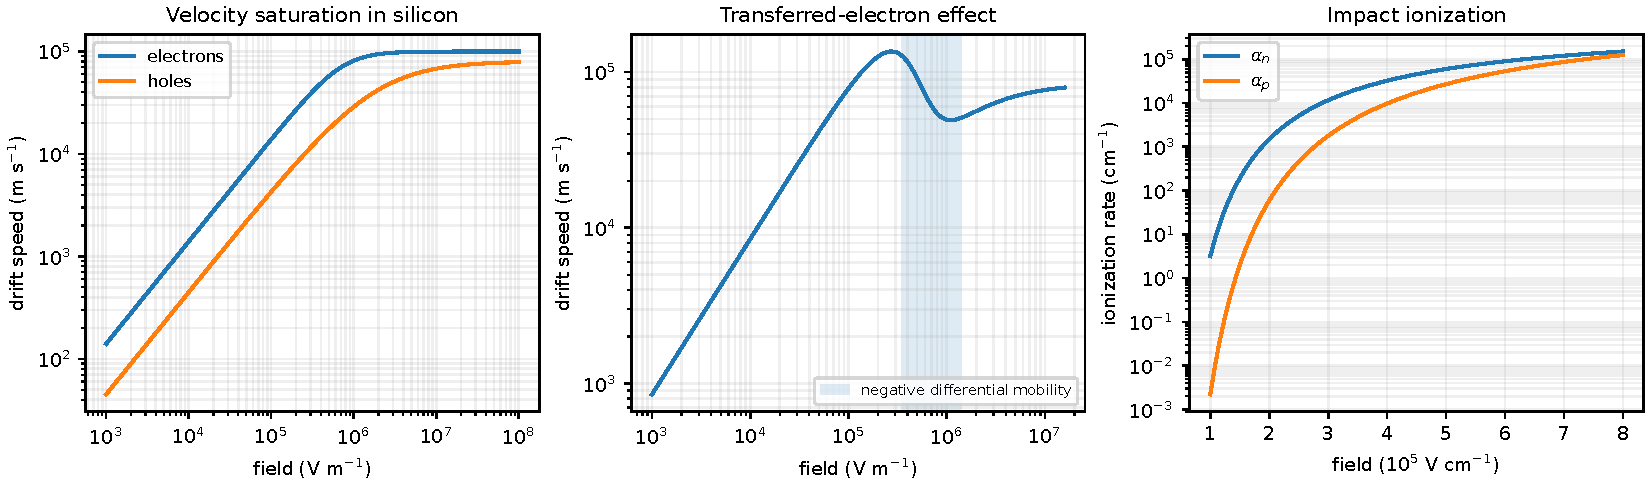
\includegraphics[width=\textwidth]{figures/transport-high-field.pdf}
  \caption{Velocity saturation in silicon, negative differential mobility from
  intervalley transfer, and the rapid field activation of electron and hole
  impact-ionization coefficients.\figurenotebookmark}
  \label{fig:transport-high-field}
\end{figure}
\figurenotebooktext{figures/15_high-field-transport/fig_15_01.ipynb}

\section{Transport-regime hierarchy}

The field scale must be compared with material and device scales.  Linear
response requires $v_d\ll v_s$.  Velocity saturation requires a field-dependent
constitutive law.  Transferred-electron transport requires multiple valleys and
an energy-dependent population model.  Impact ionization requires carrier
energy gain large enough to create pairs and must be included in continuity.
Strong carrier heating requires an energy-balance or Boltzmann description.
Quantum-coherent short structures require a transmission-based model rather
than a local velocity law.

\section{Chapter summary}

High fields invalidate constant mobility.  Silicon approaches a saturation
velocity as inelastic scattering removes field-supplied energy.  Multivalley
materials can show negative differential mobility when carriers transfer to a
low-mobility satellite valley.  Still larger fields activate impact ionization,
which adds a nonlinear generation term to carrier continuity.  These mechanisms
complete the Chapter~2 transport sequence and provide the physical inputs for
junction current, depletion-region generation, and breakdown.
